
\documentclass[12pt,a4paper]{article}

\usepackage{pdflscape}
\setlength{\textwidth}{165mm}
\setlength{\textheight}{235mm}
\setlength{\oddsidemargin}{-0mm}
\setlength{\topmargin}{-10mm}

\usepackage{mathtools}
\DeclarePairedDelimiter\abs{\lvert}{\rvert}%
\DeclarePairedDelimiter\norm{\lVert}{\rVert}%
% Swap the definition of \abs* and \norm*, so that \abs
% and \norm resizes the size of the brackets, and the
% starred version does not.
\makeatletter
\let\oldabs\abs
\def\abs{\@ifstar{\oldabs}{\oldabs*}}
%
\let\oldnorm\norm
\def\norm{\@ifstar{\oldnorm}{\oldnorm*}}
\makeatother	

\newcommand*{\Value}{\frac{1}{2}x^2}%
%\usepackage{graphicx}
\usepackage{graphicx}
\usepackage{subfigure}%exclusive to subcaption
%\usepackage{subcaption, float} 
\usepackage{xcolor}
\definecolor{ggray}{RGB}{47,79,79}
\definecolor{firebrick}{RGB}{178,34,34}
\definecolor{green1}{RGB}{50,205,50}
\definecolor{umbrella}{RGB}{0,191,255}

\usepackage{pgfplots}
\usepackage{tikz}
\usetikzlibrary{patterns,arrows,shapes,positioning,shadows,trees}
\tikzstyle{every node}=[draw=black,thick,anchor=west]
\tikzstyle{selected}=[draw=red,fill=red!30]
\tikzstyle{optional}=[dashed,fill=gray!50]
\tikzstyle{neglected}=[dashed]

\usepackage{amsfonts}
\usepackage{amssymb,amsmath} %  $\displaystyle \sum$ will print a bigger one Σ , like in equations  in amsmath package

\DeclareMathOperator{\sgn}{sgn}

\usepackage{soul}

\usepackage{titlesec}
\titleformat*{\section}{\Large\sffamily}
\titleformat*{\subsection}{\large\sffamily}
\titleformat*{\subsubsection}{\itshape \sffamily}


%\renewcommand{\refname}{參考文獻}
\usepackage[nottoc]{tocbibind}
%\settocbibname{參考文獻}

\usepackage{multirow}
\usepackage{booktabs}
%\usepackage[square]{natbib}

\title{Cloud Programming HW03}
\author{Ming-Chang Chiu 100060007}
\date{\today}
\begin{document}
\maketitle
\fontsize{12}{20pt}\selectfont %本行指令第一個12是字體大小、第二個20是行距,selectfont一定要加才會發生效果。但此指令只對正文有效,註解無效

\section{Introduction}
In this assignment, we are required to implement PageRank algorithm to construct a search engine which can prioritize the related links when we type in a keyword. 

\section{System Details: Algorithms}
In total, I wrote four MapReduce phases to complete this assignment, including graph building, inverted index building, rank computing, result sorting. In addition, I implement four HDFS, HBase manipulation programs to help me get the desired output.

As for the implementation of PageRank on MapReduce framework, I simply follow the flow as follow:
\begin{figure}[h!]
  \centering
     \includegraphics[width=1.0\textwidth]{./pralgo.png}
\end{figure}

The tricky part is, when dealing with dangling node, we could have difficulty broadcasting the sum of the score of all dangling nodes to all other running tasks. My solution is, first we create a file, say, info.txt to store the sum of dangling nodes and the total page number which the input file has, and when we need the information of them, we then just read the info.txt and then do the calculation. And after the iteration, we shall update the info.txt with newest sum of dangling nodes.

One trick worths mentioning is, when both killing non-existent nodes and getting sum of dangling nodes, we can attach a symbol as the node's value. By recognizing the symbol in the later phases, we can easily discern the status of the node, and the do the appropriate processes.
\section{Usage}

Basically, just execute scripts that I wrote and then one can acquire the desired output. Please follow the order below:
\begin{description}  
\item[invertedindex.sh:] Build the inverted index for each word in the input's <text> tag.
\item[graph.sh:] Build the interconnected graph for page titles.
\item[clean.sh:] Clean the non-existent pages in the graph. 
\item[rank.sh:] Perform the PageRank algorithm.
\item[sort.sh:] Get the output of PageRank and then output the <Page, Score> pairs sorted by score.
\item[upload.sh:] Load the inverted index and sorted PageRank to HBase. Tables are named as \verb|100060007_invertedindex|, \verb|100060007_pagerank|.
\item[query.sh:] This is the search engine that can accept keyword. The engine will first access the invertedindex in HBase, get the corresponding pages, and then get the rank for each page, and then finally print the pages sorted by rank score.
\end{description}

{\bf Notice:} In order to run correctly on each directory, one should check those 4 .sh files for the directory names. And one should modify the retrieval/ReadFile.java for the HDFS paths. The above description is based on my working directory on Quanta006.


\section{Experiment}
I perform PageRank over the 100M input file and the following is the result I got.
\begin{figure}[h!]
  \centering
     \includegraphics[width=0.8\textwidth]{./sorted.png}
     \caption{Distribution of score}
\end{figure}

\begin{figure}[h!]
  \centering
     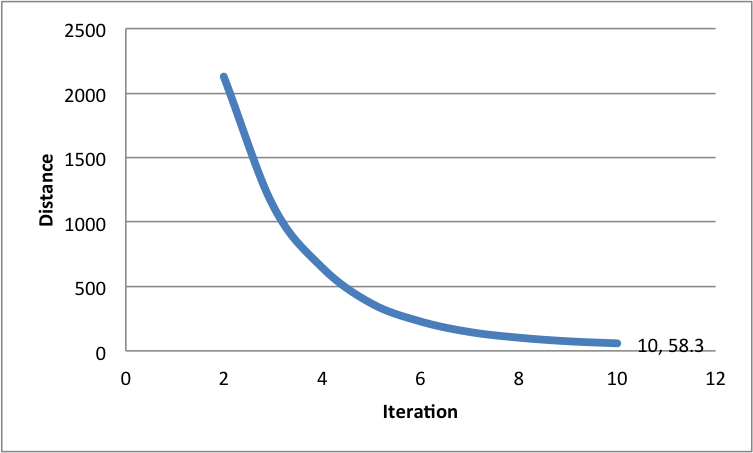
\includegraphics[width=0.8\textwidth]{./distance.png}
     \caption{Distance}
\end{figure}


\section{Observation}

In general, from $figure 1$, we can see that the distribution of rank score will decay exponentially. The distribution of iteration 5 and 10 are really close, which can be a sign of convergence. 
From $figure 2$, we see that the distance will also exponentially decline, which means the scores will fast be convergent after not too many iteration, where the definition of distance is defined as $\sum\limits_{i=1}^N |PR_i - PR_{i-1}| $.

 
\end{document}
